\frame{
\frametitle{Inertial Particles and Turbulence}

\begin{textblock*}{55mm}[0,0](0mm,0mm)
	\centering
	\only<1-2>{
		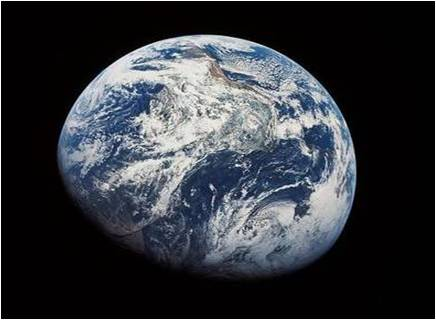
\includegraphics[height=40mm]{atm.jpg}
	}
\end{textblock*}

\begin{textblock*}{55mm}[0,0](60mm,0mm)
	\centering
	\only<1-2>{
		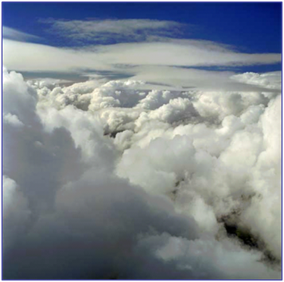
\includegraphics[height=40mm]{Nuages.png}
	}
\end{textblock*}

\begin{textblock*}{55mm}[0,0](25mm,44mm)
	\centering
	\only<2>{
		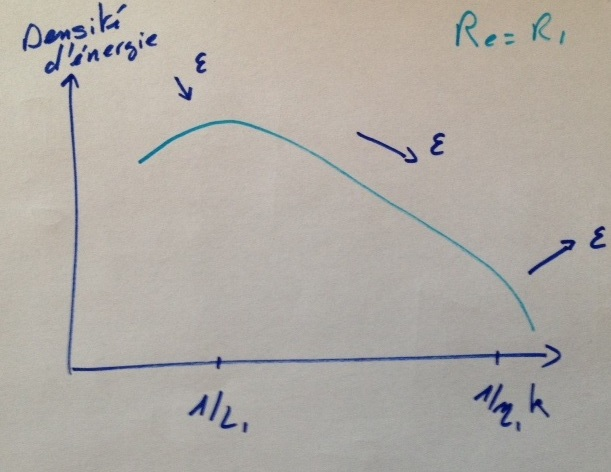
\includegraphics[width=\textwidth]{specTBL1.JPG}
	}
\end{textblock*}



\begin{textblock*}{55mm}[0,0](-5mm,0mm)
	\centering
	\only<3-5,8>{	
%		Density: $\rho_p\neq \rho_f$\\[6pt]
		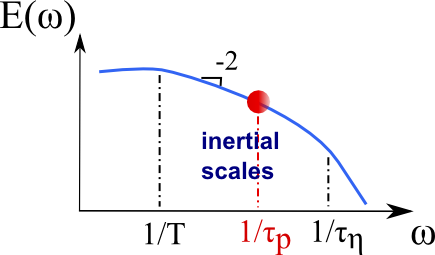
\includegraphics[width=\textwidth]{pseudoSpectre2.png}
	}
\end{textblock*}


\begin{textblock*}{55mm}[0,0](65mm,3mm)
	\only<5>{\textbf{\textcolor{myred}{Response time:}}	\\[4pt]
{\small	Stokes drag: $\tau_p = \rho_p d_p^2 / 18\mu$\\[2pt]
	Non linear drag: $\tau_p^{eff}(|\mathbf{w}|)$\\[2pt]
	Added mass: $\tau_p^{am}$\\[2pt]
	Basset history: \ldots
}}
\end{textblock*}
%
%
\begin{textblock*}{55mm}[0,0](-5mm,0mm)
	\centering
	\only<6-7>{	
		%		Density: $\rho_p\neq \rho_f$\\[6pt]
		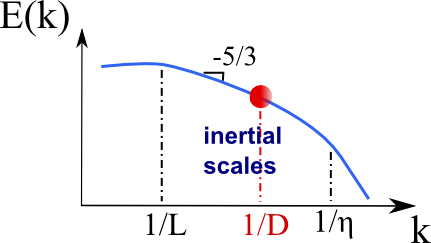
\includegraphics[width=\textwidth]{pseudoSpectre1.png}
	}
\end{textblock*}


\begin{textblock*}{55mm}[0,0](55mm,0mm)
	\centering
	\only<8->{	
		%		Size: $\eta < D < L$\\[6pt]
		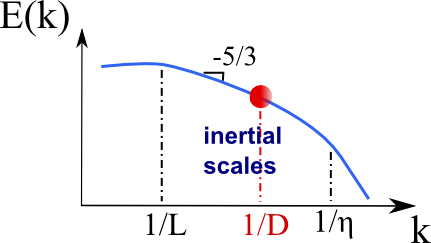
\includegraphics[width=\textwidth]{pseudoSpectre1.png}}
\end{textblock*}
%
%
\begin{textblock*}{90mm}[0,0](-5mm,37mm)
	\only<7>
	{\small{\textbf{Finite size effects:}}
	\begin{itemize}
		\item Fax\'en corrections ($d_p\leq \eta$)
		\item Filtering of small scales, integration over particle size
		\item Anisotropy
		\begin{itemize}
		\item Rotation / tumbling inertia
	\item Porosity and roughness
		\end{itemize}
		\item \ldots
	\end{itemize}
	}
\end{textblock*}
%
\begin{textblock*}{90mm}[0,0](-5mm,34mm)
	\only<8>{
{\footnotesize
\renewcommand{\arraystretch}{1.4}
\begin{tabular}{lll}
	\textbf{Source} & \textbf{Timescale} & \textbf{Relevant when} \\
	\midrule
	\rowcolor{rowlight}
	Stokes drag & $\tau_p = \rho_p d_p^2 / 18\mu$ & Always, baseline \\
	\rowcolor{rowdark}
	Nonlinear drag & $\tau_p^{eff}(|\mathbf{w}|)$ & $Re_p \gtrsim 1$ \\
	\rowcolor{rowlight}
	Added mass & $\tau_p^{am}$ & $\rho_p / \rho_f \sim \mathcal{O}(1)$ \\
	\rowcolor{rowdark}
	Basset history &complex kernel & Unsteady $\mathbf{w}$, $\rho_p / \rho_f$ moderate \\
	\rowcolor{rowlight}
	Orientational inertia & $\tau_{rot}$ & Non-spherical particles \\
	\rowcolor{rowdark}
	Finite size filtering & $d_p / \eta$ & $d_p \gtrsim \eta$ \\
	\rowcolor{rowlight}
	Porosity/permeability & Internal flow timescale & Aggregates, flocs \\
	\bottomrule
\end{tabular}
}
	}
\end{textblock*}
%
\begin{textblock*}{90mm}[0,0](-5mm,37mm)
	\only<4-5>
	{\small{\textbf{Model point particle equation:}}
		\scriptsize{
			\begin{eqnarray*}
				\rho_p\frac{\partial v_i}{\partial t}
				&=&
				% gravity
				\overbrace{
					(\rho_p-\rho_f)g_i}
				^{\mathrm{gravity}}
				% undisturbed flow
				+ \overbrace{
					\frac{\partial \tau _{ij}}{\partial x_j}	
					-\frac{\partial p}{\partial x_i}
				}
				^{\mathrm{undisturbed\ flow}}
				% steady state drag
				+\overbrace{
					\frac{9}{2}\frac{\mu}{r_p^2}\biggl (
					(u_i-v_i) + \frac{r_p^2}{6} {\nabla} ^2u_i
					\biggr)
				}
				^{\mathrm{steady\ state\ drag}}\\
				&&+
				% virtual or apparent mass term
				\overbrace{
					\frac{1}{2}\rho_f \frac{d}{dt}\biggl (
					(u_i-v_i)+ \frac{r_p^2}{10}\nabla^2u_i
					\biggr)
				}
				^{\mathrm{virtual\ or\ apparent\ mass\ term}}
				+
				% Basset history term
				\overbrace{
					\frac{24 \mu}{r_p}\int_0^t\frac{d/dt\biggl(
						u_i-v_i+r_p^2/6\nabla^2u_i
						\biggr)}
					{\pi \nu (t-\tau)^{1/2}}d\tau
				}
				^{\mathrm{Basset\ history\ term}}
			\end{eqnarray*}
	}}
\end{textblock*}
\begin{textblock*}{30mm}[0,0](77mm,76mm)
	\only<4-5>{\tiny{\begin{flushright}
				Maxey \& Riley, \textit{POF}, 26, \textbf{1983}\\
				Gattignol, \textit{JMTA}, 2, \textbf{1983} 
			\end{flushright}
	}}
\end{textblock*}  

}
